\documentclass[diss,capa]{texufpel}

\usepackage[utf8]{inputenc} % acentuacao
\usepackage{graphicx} % para inserir figuras
\usepackage[T1]{fontenc}

\hypersetup{
    hidelinks, % Remove coloração e caixas
    unicode=true,   %Permite acentuação no bookmark
    linktoc=all %Habilita link no nome e página do sumário
}

\unidade{Centro de Desenvolvimento Tecnológico}
\programa{Programa de Pós-Graduação em Computação}
\curso{Ciência da Computação}

\unidadeeng{Technology Development Center}
\programaeng{Postgraduate Program in Computing}
\cursoeng{Computer Science}

\title{Um Blabla Blablabla com Aplicações em Blablabla}

\author{Aguiar}{Marilton Sanchotene de}
\advisor[Prof.~Dr.]{Aguiar}{Marilton Sanchotene de}
\coadvisor[Prof.~Dr.]{Aguiar}{Marilton Sanchotene de}
\collaborator[Prof.~Dr.]{Aguiar}{Marilton Sanchotene de}

%Palavras-chave em PT_BR
\keyword{Palavrachave-um}
\keyword{Palavrachave-dois}
\keyword{Palavrachave-tres}
\keyword{Palavrachave-quatro}

%Palavras-chave em EN_US
\keywordeng{Keyword-one}
\keywordeng{Keyword-two}
\keywordeng{Keyword-three}
\keywordeng{Keyword-four}

\begin{document}

%\renewcommand{\advisorname}{Orientadora}           %descomente caso tenhas orientadora
%\renewcommand{\coadvisorname}{Coorientadora}      %descomente caso tenhas coorientadora

\maketitle 

\sloppy

\fichacatalografica

%Composição da Banca Examinadora
\begin{aprovacao}{30 de fevereiro de 2019} %data da banca por extenso
\noindent Prof. Dr. Marilton Sanchotene de Aguiar (orientador)\\
Doutor em Computação pela Universidade Federal do Rio Grande do Sul.\\[1cm]

\noindent Prof. Dr. Paulo Roberto Ferreira Jr.\\
Doutor em Computação pela Universidade Federal do Rio Grande do Sul.\\[1cm]

\noindent Prof. Dr. Ricardo Matsumura Araujo\\
Doutor em Computação pela Universidade Federal do Rio Grande do Sul.\\[1cm]

\noindent Prof. Dr. Luciano da Silva Pinto\\
Doutor em Biotecnologia pela Universidade Federal de Pelotas.
\end{aprovacao}

%Opcional
\begin{dedicatoria}
  Dedico\ldots 
\end{dedicatoria}

%Opcional
\begin{agradecimentos}
  Agradeço\ldots 
\end{agradecimentos}

%Opcional
\begin{epigrafe}
  Só sei que nada sei.\\
  {\sc --- Sócrates}
\end{epigrafe}

%Resumo em Portugues (no maximo 500 palavras)
\begin{abstract}
Bla blabla blablabla bla.  Bla blabla blablabla bla.  Bla blabla
blablabla bla.  Bla blabla blablabla bla.  Bla blabla blablabla bla.
Bla blabla blablabla bla.  Bla blabla blablabla bla.  Bla blabla
blablabla bla.  Bla blabla blablabla bla.  Bla blabla blablabla bla.
Bla blabla blablabla bla.  Bla blabla blablabla bla.  Bla blabla
blablabla bla.  Bla blabla blablabla bla.  Bla blabla blablabla bla.
Bla blabla blablabla bla.  Bla blabla blablabla bla.  Bla blabla
blablabla bla.  Bla blabla blablabla bla.  Bla blabla blablabla bla.
Bla blabla blablabla bla.
\end{abstract}

%Resumo em Inglês (no maximo 500 palavras)
\begin{englishabstract}{Titulo do Trabalho em Ingles}
Bla blabla blablabla bla.  Bla blabla blablabla bla.  Bla blabla
blablabla bla.  Bla blabla blablabla bla.  Bla blabla blablabla bla.
Bla blabla blablabla bla.  Bla blabla blablabla bla.  Bla blabla
blablabla bla.  Bla blabla blablabla bla.  Bla blabla blablabla bla.
Bla blabla blablabla bla.  Bla blabla blablabla bla.  Bla blabla
blablabla bla.  Bla blabla blablabla bla.  Bla blabla blablabla bla.
Bla blabla blablabla bla.  Bla blabla blablabla bla.  Bla blabla
blablabla bla.  Bla blabla blablabla bla.  Bla blabla blablabla bla.
Bla blabla blablabla bla.
\end{englishabstract}

%Lista de Figuras
\listoffigures

%Lista de Tabelas
\listoftables

%lista de abreviaturas e siglas
\begin{listofabbrv}{ABNT}%coloque aqui a maior sigla para ajustar a distância
        \item[ABNT] Associação Brasileira de Normas Técnicas
        \item[NUMA] Non-Uniform Memory Access
        \item[SIMD] Single Instruction Multiple Data
        \item[SMP] Symmetric Multi-Processor
        \item[SPMD] Single Program Multiple Data
\end{listofabbrv}

%Sumario
\tableofcontents

\chapter{Introdução}

\section{Uma subseção}
Bla blabla blablabla bla.  Bla blabla blablabla bla.  Bla blabla
blablabla bla.  Bla blabla blablabla bla.  Bla blabla blablabla bla.
Bla blabla blablabla bla.  Bla blabla blablabla bla.  Bla blabla
blablabla bla.  Bla blabla blablabla bla.  Bla blabla blablabla bla.
Bla blabla blablabla bla.  Bla blabla blablabla bla.  Bla blabla
blablabla bla.  Bla blabla blablabla bla.  Bla blabla blablabla bla.
Bla blabla blablabla bla.  Bla blabla blablabla bla.  Bla blabla
blablabla bla.  Bla blabla blablabla bla.  Bla blabla blablabla bla.
Bla blabla blablabla bla.

Bla blabla blablabla bla.  Bla blabla blablabla bla.  Bla blabla
blablabla bla.  Bla blabla blablabla bla.  Bla blabla blablabla bla.
Bla blabla blablabla bla.  Bla blabla blablabla bla.  Bla blabla
blablabla bla.  Bla blabla blablabla bla.  Bla blabla blablabla bla.
Bla blabla blablabla bla.  Bla blabla blablabla bla.  Bla blabla
blablabla bla.  Bla blabla blablabla bla.  Bla blabla blablabla bla.
Bla blabla blablabla bla.  Bla blabla blablabla bla.  Bla blabla
blablabla bla.  Bla blabla blablabla bla.  Bla blabla blablabla bla.
Bla blabla blablabla bla~\citet{Moore:1979:MAI,Aguiar:2005}.

Bla blabla blablabla bla.  Bla blabla blablabla bla.  Bla blabla
blablabla bla.  Bla blabla blablabla bla.  Bla blabla blablabla bla.
Bla blabla blablabla bla.  Bla blabla blablabla bla.  Bla blabla
blablabla bla.  Bla blabla blablabla bla.  Bla blabla blablabla bla.
Bla blabla blablabla bla.  Bla blabla blablabla bla.  Bla blabla
blablabla bla.  Bla blabla blablabla bla.  Bla blabla blablabla bla.
Bla blabla blablabla bla.  Bla blabla blablabla bla.  Bla blabla
blablabla bla.  Bla blabla blablabla bla.  Bla blabla blablabla bla.
Bla blabla blablabla bla~\cite{vonNeumann:1966:TSR}.

\section{Outra seção}

Bla blabla blablabla bla.  Bla blabla blablabla bla.  Bla blabla
blablabla bla.  Bla blabla blablabla bla.  Bla blabla blablabla bla.
Bla blabla blablabla bla.  Bla blabla blablabla bla.  Bla blabla
blablabla bla.  Bla blabla blablabla bla.  Bla blabla blablabla bla.
Bla blabla blablabla bla.  Bla blabla blablabla bla.  Bla blabla
blablabla bla.  Bla blabla blablabla bla.  Bla blabla blablabla bla.
Bla blabla blablabla bla.  Bla blabla blablabla bla.  Bla blabla
blablabla bla.  Bla blabla blablabla bla.  Bla blabla blablabla bla.
Bla blabla blablabla bla~\ref{tabela}.

\begin{table}
  \begin{center}
    \caption{Nome da Tabela}\label{tabela}
    \begin{tabular}{p{4cm}p{5cm}p{6cm}}
      \hline
      Blabla & Blabla & Blablabla\\
      \hline
      {\small Bla} & {\small Blabla} & {\small\em Bla blabla blablabla blabla
        blablabla blabla blablabla.}\\
      {\small Bla} & {\small Blabla} & {\small\em Bla blabla blablabla blabla
        blablabla blabla blablabla.}\\
      {\small Bla} & {\small Blabla} & {\small\em Bla blabla blablabla blabla
        blablabla blabla blablabla.}\\
      {\small Bla} & {\small Blabla} & {\small\em Bla blabla blablabla blabla
        blablabla blabla blablabla.}\\
      {\small Bla} & {\small Blabla} & {\small\em Bla blabla blablabla blabla
        blablabla blabla blablabla.}\\
      {\small Bla} & {\small Blabla} & {\small\em Bla blabla blablabla blabla
        blablabla blabla blablabla.}\\
      \hline
    \end{tabular}
  \end{center}
\end{table}

\subsection{Uma subseção}

Bla blabla blablabla bla.  Bla blabla blablabla bla.  Bla blabla
blablabla bla.  Bla blabla blablabla bla.  Bla blabla blablabla bla.
Bla blabla blablabla bla.  Bla blabla blablabla bla.  Bla blabla
blablabla bla.  Bla blabla blablabla bla.  Bla blabla blablabla bla.
Bla blabla blablabla bla.  Bla blabla blablabla bla.  Bla blabla
blablabla bla.  Bla blabla blablabla bla.  Bla blabla blablabla bla.
Bla blabla blablabla bla.  Bla blabla blablabla bla.  Bla blabla
blablabla bla.  Bla blabla blablabla bla.  Bla blabla blablabla bla.
Bla blabla blablabla bla.

\chapter{Desenvolvimento}

  Bla blabla blablabla bla.  Bla blabla blablabla bla.  Bla blabla
  blablabla bla.  Bla blabla blablabla bla.  Bla blabla blablabla bla.
  Bla blabla blablabla bla.  Bla blabla blablabla bla.  Bla blabla
  blablabla bla.  Bla blabla blablabla bla.  Bla blabla blablabla bla.
  Bla blabla blablabla bla.  Bla blabla blablabla bla.  Bla blabla
  blablabla bla.  Bla blabla blablabla bla.  Bla blabla blablabla bla.
  Bla blabla blablabla bla.  Bla blabla blablabla bla.  Bla blabla
  blablabla bla.  Bla blabla blablabla bla.  Bla blabla blablabla bla.
  Bla blabla blablabla bla~\ref{tabela2}.

\begin{table}
\begin{center}
\caption{Nome da Tabela}\label{tabela2}
\begin{tabular}{p{4cm}p{5cm}p{6cm}}
\hline
Blabla & Blabla & Blablabla\\
\hline
{\small Bla} & {\small Blabla} & {\small\em Bla blabla blablabla blabla
  blablabla blabla blablabla.}\\
{\small Bla} & {\small Blabla} & {\small\em Bla blabla blablabla blabla
  blablabla blabla blablabla.}\\
{\small Bla} & {\small Blabla} & {\small\em Bla blabla blablabla blabla
  blablabla blabla blablabla.}\\
{\small Bla} & {\small Blabla} & {\small\em Bla blabla blablabla blabla
  blablabla blabla blablabla.}\\
{\small Bla} & {\small Blabla} & {\small\em Bla blabla blablabla blabla
  blablabla blabla blablabla.}\\
{\small Bla} & {\small Blabla} & {\small\em Bla blabla blablabla blabla
  blablabla blabla blablabla. Conforme a figura~\ref{figura}}\\
\hline
\end{tabular}
\end{center}
\end{table}

\begin{figure}[htbp]
  \centering \includegraphics[scale=.4]{figura}
\caption{Nome da figura} 
\label{figura}
\end{figure}



\chapter{Metodologia}
% (ENTRE 1 e 3 PÁGINAS)

% O processo de mineração de dados envolve várias fases e etapas. Este trabalho classifica o processo de KDD em três grandes fases, com base nas abordagens descritas em [Silva and Vieira 2002] e [Rezende et al. 2003]: Preparação, Extração de Padrões e Pós-Processamento. Cada fase pode envolver uma ou mais etapas conforme mostra a tabela 1. No entanto, o KDD é um processo iterativo e algumas etapas podem ser realizadas novamente após a análise dos padrões encontrados de forma a melhorá-los \cite{Pimentel2006}.

Neste trabalho será utilizado uma metodologia apresentada no livro de \citet{goldschmidt2015data}, que é baseada na metodologia CRISP-DM (Cross-Industry Standard Process for Data Mining) e em alguns princípios de planejamento de atividades. A metodologia mostrada no livro se difere da metodologia CRISP-DM no momento em que ela sugere aplicar a definição dos objetivos e escolha da técnica de mineração antes da faze de preparação dos dados. Além disso, ela adiciona instrumentos para documentar as decisões e os resultados durante o processo de KDD, um exemplo é o formulário mostrado na figura \ref{fig:formulario-para-documentacao-de-acoes}.

\begin{figure}[htbp]
  \centering 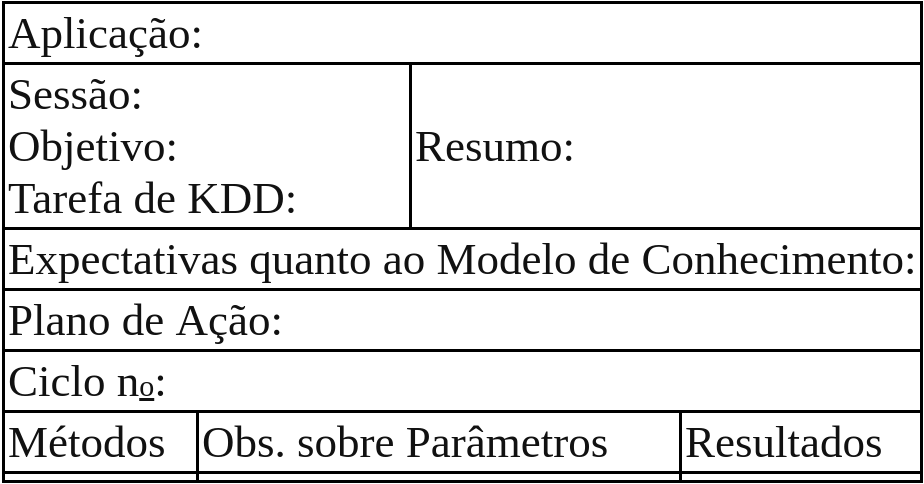
\includegraphics[scale=.4]{imagens/formulario-para-documentacao-de-acoes.png}
  \caption{Formulário para documentação de ações \cite{goldschmidt2015data}.}
  \label{fig:formulario-para-documentacao-de-acoes}
\end{figure}

A metodologia proposta no livo divide o processo em 5 etapas Levantamento da Situação Vigente, Definição dos Objetivos, Planejamento de Atividades, Execução dos Planos de Ação e Avaliação de Resultados. O resto desta sessão aprofunda cada uma dessas etapas.

\section{Levantamento da Situação Vigente}
\label{sec:levantamento-da-situacao-vigente}

Nesta etapa deve ser realizada todas as fases da \textbf{Compreensão do Negócio} e \textbf{Compreensão dos Dados} da metodologia CRISP-DM. 

A fase de \textbf{Compreensão do Negócio} tem como meta compreender o contexto em que o processo de KDD será realizado. As principais considerações técnicas desta fase são:
\begin{itemize}
\item Fazer a identificação das pessoas envolvidas no processo;
\item Elaborar uma lista de necessidades e expectativas das pessoas envolvidas quanto ao propósito do KDD;
\item Conhecer o software e hardware existentes;
\item Elaborar um inventário da base de dados;
\item Verificar se existe um Data Warehouse;
\item Tentar identificar e documentar todo o conhecimento prévio existente e disponível sobre o domínio da aplicação.
\end{itemize}

Na fase de \textbf{Compreensão dos dados} será feito um estudo detalhado das informações disponíveis. Esta fase vão ser realizadas as etapas destacadas abaixo:
\begin{itemize}
\item Compreender como um todo os dados e atributos disponíveis da base de dados;
\item Avaliar a qualidade dos dados disponíveis;
\item Verificar a disponibilidade dos dados, principalmente sobre a quantidade dos dados;
\end{itemize}

Já na etapa de levantamento vai ser usado o formulário da figura \ref{formulario-para-documentacao-de-acoes} para documentação de ações e resultados do processo de KDD. O formulário deve ser utilizado para registrar o titulo da aplicação e um resumo descritivo do trabalho.


% É nesta etapa que será realizado um estudo mais aprofundado para tentar entender mais a fundo o problema da evasão e também tentar definir o objetivo sob a luz de descoberta de conhecimento em base de dados.

\section{Definição dos Objetivos}
\label{sec:definicao-dos-objetivos}

Na metodologia proposta do livro a etapa de Definição dos Objetivos agrega duas fazes da metodologia CRISP-DM Compreensão do Negócio e Modelagem. Essa etapa destaca que a escolha da técnica mineração deve vir antes da preparação dos dados, logo o pré-processamento dos dados pode seguir em função da técnica de mineração aplicada aos dados.

De forma prática primeiramente serão identificadas todas as expectativas, logo depois elas serão validadas junto aos Orientadores. Por fim, essas expectativas serão agrupadas de acordo com sua natureza e de forma que um modelo de conhecimento possa englobar um grupo de expectativas.

Com as expectativas identificas e agrupadas será apurado qual tipo de tarefa de Mineração de Dados deve ser aplicado para obter um modelo de conhecimento que atenda a cada grupo de expectativa.

Nesta etapa serão preenchidos os seguintes campos do formulário gerado na etapa anterior: Sessão, Objetivo, Tarefa de KDD e Expectativas quanto ao modelo de conhecimento.
Uma sessão estará associada a uma única tarefa de KDD. O objetivo será associado a um grupo de expectativas. A tarefa de KDD será a tarefa que será executada para o objetivo dessa sessão. Para o ultimo campo será especificado uma lista de expectativas quanto ao modelo de conhecimento.

A figura~\ref{fig:formulario-etapa-definicao-objetivo} é um exemplo de como preencher o formulário da sessão \ref{sec:levantamento-da-situacao-vigente}. É o exemplo da expectativa de comportamento do cliente que é mapeada em uma tarefa de Descoberta de Sequência.

\begin{figure}[htbp]
  \centering 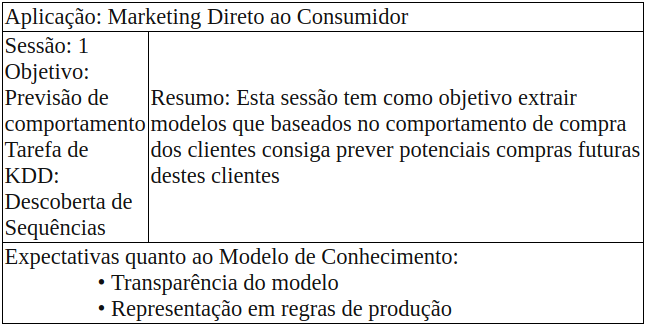
\includegraphics[scale=.4]{imagens/formulario-etapa-definicao-objetivo.png}
  \caption{Exemplo de preenchimento do formulário na etapa de Definição de Objetivos. Fonte: \cite{goldschmidt2015data}.}
  \label{fig:formulario-etapa-definicao-objetivo}
\end{figure}

\section{Planejamento de atividades}
\label{sec:planejamento-de-atividades}

Nesta etapa cada sessão de KDD identificada na sessão \ref{sec:definicao-dos-objetivos} deverá ser elaborado um planejamento de atividades que proporcione a execução do objetivo correspondente. Também será identificado, dentre o métodos disponíveis, aqueles que melhor implementam a tarefa da sessão de KDD. Este métodos são chamados de métodos candidatos.

Segundo \citet{goldschmidt2015data} a filtragem dos métodos requer conhecimento profundo de cada método e que a escolha do método depende da preferência pessoal do analista de KDD, porem ressalva que todos os métodos candidatos que não foram retirados da filtragem devem ser considerados. A filtragem dos métodos candidatos será feita junto aos orientadores e ao fim dessa filtragem será elaborado uma lista ordenada dos método que podem obter melhor resultado.

A partir da listagem dos métodos selecionados será apresentado alternativas de pré-processamento para cada método da lista. \citet{goldschmidt2015data} denomina essas alternativas de pré-processamento de planos de ação e que o analista deve planejar quais métodos de pré-processamento devem ser utilizados, incluindo a ordem de aplicação.

A figura \ref{fig:formulario-etapa-planejamento-atividades} é um exemplo retirado do livro que mostra como ficaria o formuláro após a etapa de planejamento de atividades.

\begin{figure}[htbp]
  \centering 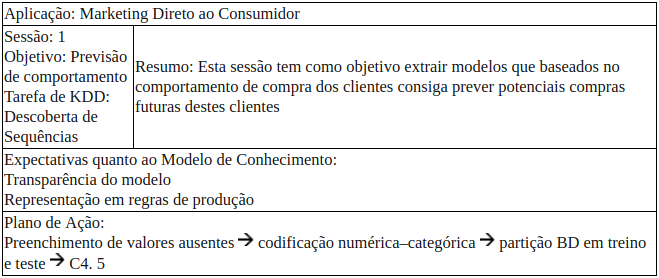
\includegraphics[scale=.4]{imagens/formulario-etapa-planejamento-atividades.png}
  \caption{Exemplo de preenchimento do formulário na etapa de Planejamento de Atividades. Fonte: \cite{goldschmidt2015data}.}
  \label{fig:formulario-etapa-planejamento-atividades}
\end{figure}

\section{Execução do Plano de Ação}
\label{sec:execucao-do-plano-de-acao}

Nesta etapa todos os planos de ação descritos na sessão \ref{sec:planejamento-de-atividades} serão experimentados e avaliados. \citet{goldschmidt2015data} recomenda que os planos sejam executados simultaneamente para ser feito uma análise conjunta dos resultados obtidos. Isso pode trazer uma visão global do processo e pode ser possível perceber detalhes que permitam reavaliar ou mudar a estratégia escolhida.

\citet{goldschmidt2015data} recomenda também que o plano de ação entende a execução ordenada dos métodos do plano e deve ser executada em ciclos. Ou seja, o plano deve ser executado total ou parcialmente a cada ciclo, procurando obter os melhores resultados.

\citet{goldschmidt2015data} destaca que um problema frequente em um processo de KDD é a escolha dos parâmetros de um algoritmo frente a uma nova situação. Este problema pode aumentar bastante o número de ciclos do processo. Por isso, nessa etapa serão registrados dos parâmetros adotados e os resultados obtidos a cada ciclo no formulário. A figura \ref{fig:formulario-etapa-execucao-dos-planos-de-acao} mostra um possível preenchimento do formulário.

\section{Avaliação de Resultados}
\label{sec:avaliacao-de-resultados}

Esta etapa deve ser realizada no final do processamento de cada método do plano. \citet{goldschmidt2015data} diz que é o momento de comparar as características do modelo de conhecimento gerado com as expectativas quanto ao modelo de conhecimento listadas na sessão \ref{sec:definicao-dos-objetivos}. Ele reforça que algumas medidas podem ser comparadas diretamente, já outras, são mais subjetivas. Uma pergunta que poderia se fazer nessa etapa é qual é a exclusividade e utilidade do conhecimento extraído? Por isso, esta etapa deverá ser homologada junto ao orientador deste trabalho. Nessa etapa também terá de ser feito um estudo sobre as medidas de interesse no processo de KDD.

\begin{figure}[htbp]
  \centering 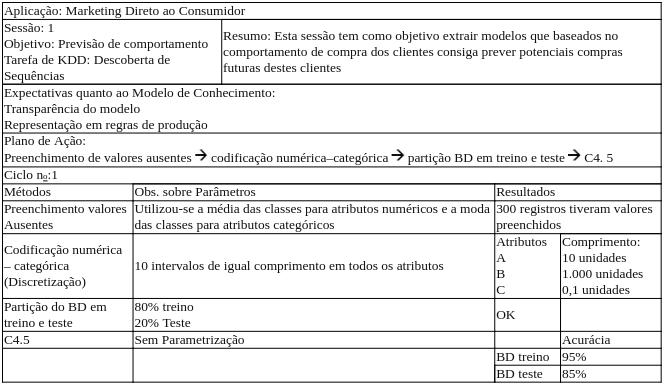
\includegraphics[scale=.4]{imagens/formulario-etapa-execucao-dos-planos-de-acao.png}
  \caption{Exemplo de preenchimento do formulário na etapa de Execução do plano de ação. Fonte: \cite{goldschmidt2015data}.}
  \label{fig:formulario-etapa-execucao-dos-planos-de-acao}
\end{figure}





\chapter{Conclusão}

Bla blabla blablabla bla.  Bla blabla blablabla bla.  Bla blabla
blablabla bla.  Bla blabla blablabla bla.  Bla blabla blablabla bla.
Bla blabla blablabla bla.  Bla blabla blablabla bla.  Bla blabla
blablabla bla.  Bla blabla blablabla bla.  Bla blabla blablabla bla.
Bla blabla blablabla bla.  Bla blabla blablabla bla.  Bla blabla
blablabla bla.  Bla blabla blablabla bla.  Bla blabla blablabla bla.
Bla blabla blablabla bla.  Bla blabla blablabla bla.  Bla blabla
blablabla bla.  Bla blabla blablabla bla.  Bla blabla blablabla bla.
Bla blabla blablabla bla.

Bla blabla blablabla bla.  Bla blabla blablabla bla.  Bla blabla
blablabla bla.  Bla blabla blablabla bla.  Bla blabla blablabla bla.
Bla blabla blablabla bla.  Bla blabla blablabla bla.  Bla blabla
blablabla bla.  Bla blabla blablabla bla.  Bla blabla blablabla bla.
Bla blabla blablabla bla.  Bla blabla blablabla bla.  Bla blabla
blablabla bla.  Bla blabla blablabla bla.  Bla blabla blablabla bla.
Bla blabla blablabla bla.  Bla blabla blablabla bla.  Bla blabla
blablabla bla.  Bla blabla blablabla bla.  Bla blabla blablabla bla.
Bla blabla blablabla bla.

% Bibliografia http://liinwww.ira.uka.de/bibliography/index.html um
% site que cataloga no formato bibtex a bibliografia em computacao
% \bibliography{nomedoarquivo.bib} (sem extensao)
% \bibliographystyle{formato.bst} (sem extensao)

\bibliographystyle{abnt}
\bibliography{bibliografia} 

% Apêndices (Opcional) - Material produzido pelo autor
\apendices
\chapter{Um Apêndice}

% Anexos (Opcional) - Material produzido por outro
\anexos
\chapter{Um Anexo}

Bla blabla blablabla bla.  Bla blabla blablabla bla.  Bla blabla
blablabla bla.  Bla blabla blablabla bla.  Bla blabla blablabla bla.
Bla blabla blablabla bla.  Bla blabla blablabla bla.  Bla blabla
blablabla bla.  Bla blabla blablabla bla.  Bla blabla blablabla bla.
Bla blabla blablabla bla.  Bla blabla blablabla bla.  Bla blabla
blablabla bla.  Bla blabla blablabla bla.  Bla blabla blablabla bla.
Bla blabla blablabla bla.  Bla blabla blablabla bla.  Bla blabla
blablabla bla.  Bla blabla blablabla bla.  Bla blabla blablabla bla.
Bla blabla blablabla bla.

Bla blabla blablabla bla.  Bla blabla blablabla bla.  Bla blabla
blablabla bla.  Bla blabla blablabla bla.  Bla blabla blablabla bla.
Bla blabla blablabla bla.  Bla blabla blablabla bla.  Bla blabla
blablabla bla.  Bla blabla blablabla bla.  Bla blabla blablabla bla.
Bla blabla blablabla bla.  Bla blabla blablabla bla.  Bla blabla
blablabla bla.  Bla blabla blablabla bla.  Bla blabla blablabla bla.
Bla blabla blablabla bla.  Bla blabla blablabla bla.  Bla blabla
blablabla bla.  Bla blabla blablabla bla.  Bla blabla blablabla bla.
Bla blabla blablabla bla.

\chapter{Outro Anexo}

Bla blabla blablabla bla.  Bla blabla blablabla bla.  Bla blabla
blablabla bla.  Bla blabla blablabla bla.  Bla blabla blablabla bla.
Bla blabla blablabla bla.  Bla blabla blablabla bla.  Bla blabla
blablabla bla.  Bla blabla blablabla bla.  Bla blabla blablabla bla.
Bla blabla blablabla bla.  Bla blabla blablabla bla.  Bla blabla
blablabla bla.  Bla blabla blablabla bla.  Bla blabla blablabla bla.
Bla blabla blablabla bla.  Bla blabla blablabla bla.  Bla blabla
blablabla bla.  Bla blabla blablabla bla.  Bla blabla blablabla bla.
Bla blabla blablabla bla.

Bla blabla blablabla bla.  Bla blabla blablabla bla.  Bla blabla
blablabla bla.  Bla blabla blablabla bla.  Bla blabla blablabla bla.
Bla blabla blablabla bla.  Bla blabla blablabla bla.  Bla blabla
blablabla bla.  Bla blabla blablabla bla.  Bla blabla blablabla bla.
Bla blabla blablabla bla.  Bla blabla blablabla bla.  Bla blabla
blablabla bla.  Bla blabla blablabla bla.  Bla blabla blablabla bla.
Bla blabla blablabla bla.  Bla blabla blablabla bla.  Bla blabla
blablabla bla.  Bla blabla blablabla bla.  Bla blabla blablabla bla.
Bla blabla blablabla bla.

% Faz a capa do CDROM
% \makecover

\end{document}

